\subsection{Membres de groupe}

Nous sommes trois étudiants du groupe M2 :
\begin{dinglist}{111}
    \item Ying LIU
    \item Philippe NEGREL-JERZY
    \item Sébastien PONT
\end{dinglist}

\subsection{Présentation}

Nous ne représentons pas tout le sujet (que vous pouvez retrouver \href{https://spont.me/mjxoog}{ici}\footnote{\href{https://spont.me/mjxoog}{https://spont.me/mjxoog}}), mais voici un résumé.

Linda est un service permettant de partager des données sous formes de \iCode{Tuple}.
Dans ce projet nous allons implémenter deux manières de partager et gérer ces ressources à travers plusieurs clients :

\begin{itemize}
    \item une version dite "locale" à base de mémoire partagée (\iCode{shm} package Figure \ref{fig:main_class_diagram})
    \item une version dite "distante" à base de clients / monoserveur (\iCode{server} package Figure \ref{fig:main_class_diagram})
\end{itemize}

\begin{figure}[H]
    \centering
    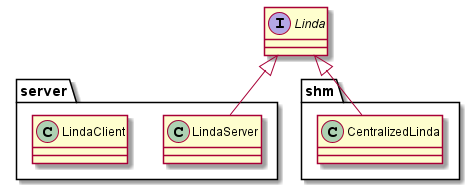
\includegraphics[scale=0.7]{src/part-01/mainCD.png}
    \caption{Diagramme de classe général du projet} \label{fig:main_class_diagram}
\end{figure}

\begin{dinglist}{111}
    \item Version mémoire partagée (version locale) : Chaque client est un nouveau \textit{thread}.
    \item Version client / monoserveur (version distante) : Un serveur tourne et communique via \textit{RMI} aux différents clients.
\end{dinglist}


\subsection{Gradle}

Pour simplifier la gestion des dépendances et faciliter le développement nous avons choisi d'utiliser
l'outil \textit{Gradle} \footnote{\href{https://gradle.org/}{gradle.org}}.
Ainsi, pour compiler le programme, il suffit par exemple de taper dans un terminal à la racine du projet :

\sFF{src/part-01/com.cmd}{Lancer l'application java via Gradle}{gradle-run}